\documentclass{beamer}
\usepackage{fontspec}
\usepackage{polyglossia}
\setmainlanguage{german}
%\setotherlanguage{greek}
\usepackage{xparse}
\usepackage{mymath}
\usepackage{stmaryrd}

\usetheme{Luebeck}
\setbeamertemplate{theorems}[normal font]
\newtheorem{satz}[theorem]{Satz}

\usepackage{wasysym}
% http://tex.stackexchange.com/questions/55806/mindmap-tikzpicture-in-beamer-reveal-step-by-step/55849#55849
  % Keys to support piece-wise uncovering of elements in TikZ pictures:
  % \node[visible on=<2->](foo){Foo}
  % \node[visible on=<{2,4}>](bar){Bar}   % put braces around comma expressions
  %
  % Internally works by setting opacity=0 when invisible, which has the 
  % adavantage (compared to \node<2->(foo){Foo} that the node is always there, hence
  % always consumes space that (foo) is always available.
  %
  % The actual command that implements the invisibility can be overriden
  % by altering the style invisible. For instance \tikzsset{invisible/.style={opacity=0.2}}
  % would dim the "invisible" parts. Alternatively, the color might be set to white, if the
  % output driver does not support transparencies (e.g., PS) 
  %
  \tikzset{
    invisible/.style={opacity=0},
    visible on/.style={alt={#1{}{invisible}}},
    alt/.code args={<#1>#2#3}{%
      \alt<#1>{\pgfkeysalso{#2}}{\pgfkeysalso{#3}} % \pgfkeysalso doesn't change the path
    },
  }
\DeclareDocumentCommand{\dilate}{}{\oplus}
\DeclareDocumentCommand{\erode}{}{\ominus}
\DeclareDocumentCommand{\open}{}{\mathbin{\Circle}}
\DeclareDocumentCommand{\close}{}{\mathbin{\CIRCLE}}
\DeclareDocumentCommand{\openclose}{}{\mathbin{\rotatebox[origin=c]{-90}{\RIGHTcircle}}}
\DeclareDocumentCommand{\closeopen}{}{\mathbin{\rotatebox[origin=c]{90}{\RIGHTcircle}}}
\DeclareDocumentCommand{\wtophat}{}{\sqcap}
\DeclareDocumentCommand{\btophat}{}{\sqcup}
\DeclareDocumentCommand{\hitormiss}{}{\circledcirc}
\DeclareDocumentCommand{\rankorder}{}{\mathbin{\diamond}}
\DeclareDocumentCommand{\sort}{}{\operatorname{sort}}
\DeclareDocumentCommand{\med}{}{\operatorname{med}}


\DeclareDocumentCommand{\veewedge}{}{\mathbin{\vee\mkern-5mu\wedge}}
\DeclareDocumentCommand{\bigveewedge}{}{\operatornamewithlimits{\bigvee\mkern-7mu\bigwedge}}
\DeclareDocumentCommand{\wbtophat}{}{\mathbin{\wtophat\mkern-1mu\btophat}}
\DeclareDocumentCommand{\bwtophat}{}{\mathbin{\btophat\mkern-1mu\wtophat}}

% http://tex.stackexchange.com/questions/117117/plus-minus-sign-in-a-circle
\newcommand{\opm}{
    \mathbin{
        \mathchoice
            {\buildcirclepm{\displaystyle     }{0.14ex}{0.95}{0.05ex}{.7}}
            {\buildcirclepm{\textstyle        }{0.14ex}{0.95}{0.05ex}{.7}}
            {\buildcirclepm{\scriptstyle      }{0.13ex}{0.955}{0.04ex}{.55}}
            {\buildcirclepm{\scriptscriptstyle}{0.08ex}{0.95}{0.03ex}{.45}}
    }
}
\newcommand{\omp}{
    \mathbin{
        \mathchoice
            {\buildcirclemp{\displaystyle     }{0.14ex}{0.95}{0.05ex}{.7}}
            {\buildcirclemp{\textstyle        }{0.14ex}{0.95}{0.05ex}{.7}}
            {\buildcirclemp{\scriptstyle      }{0.13ex}{0.955}{0.04ex}{.55}}
            {\buildcirclemp{\scriptscriptstyle}{0.08ex}{0.95}{0.03ex}{.45}}
    }
}
\newcommand\buildcirclepm[5]{%
    \begin{tikzpicture}[baseline=(X.base), inner sep=-#5, outer sep=-.65]
        \node[draw,circle,line width=#4] (X)  {\footnotesize\raisebox{#2}{\scalebox{#3}{$#1\pm$}}};
    \end{tikzpicture}%
}
\newcommand\buildcirclemp[5]{%
    \begin{tikzpicture}[baseline=(X.base), inner sep=-#5, outer sep=-.65]
        \node[draw,circle,line width=#4] (X)  {\footnotesize\raisebox{#2}{\scalebox{#3}{$#1\mp$}}};
    \end{tikzpicture}%
}

\DeclareDocumentCommand{\dilateerode}{}{\opm}
\DeclareDocumentCommand{\erodedilate}{}{\omp}


\usetikzlibrary{spy}
\tikzset{
    centerbase/.style={baseline={([yshift=-0.55ex]current bounding box.center)}},
}
\usetikzlibrary{calc}


\title{Morphologische Filter}

\author{Stephan Hilb}
\date{\today}
\institute{Universität Stuttgart}


\begin{document}


\begin{frame}
    \titlepage
\end{frame}


\section{Einführung}

\subsection{Beispiele und Motivation}

\begin{frame}
    \frametitle{Morphologische Filter}
    \begin{itemize}
        \item
            Mathematische Morphologie: Analyse räumlicher Strukturen eines Bildes
        \item
            Grundlegende morphologische Operatoren: Erosion, Dilatation
        \item
            Kompliziertere Operatoren, meist zusammengesetzt
    \end{itemize}
\end{frame}

\begin{frame}
    \frametitle{Beispiel: Dilatation}
    \begin{center}
        \pause
        \begin{onlyenv}<2-4>
            \begin{tikzpicture}[centerbase]
                \node[anchor=south west,inner sep=0] (im) at (0,0) {
\includegraphics[width=4.2cm]{images/phantom80.png}};
            \end{tikzpicture}
        \end{onlyenv}%
        \begin{onlyenv}<5->
            \begin{tikzpicture}[centerbase,spy using outlines={circle,magnification=6,size=2.5cm,connect spies}]
                \node[anchor=south west,inner sep=0] (im) at (0,0) {
\includegraphics[width=4.2cm]{images/phantom80.png}};
                \begin{scope}[x={($1/80*(im.south east)$)},y={($1/80*(im.north west)$)},xshift=0.11,yshift=-0.09]
                    \coordinate<-5> (x) at (20,59);
                    \coordinate<6> (x) at (20,60);
                    \coordinate<7> (x) at (20,61);
                    \coordinate<8> (x) at (20,62);
                    \coordinate<9> (x) at (19,62);
                    \coordinate<10> (x) at (18,62);
                    \coordinate<11> (x) at (17,62);
                    \coordinate<12> (x) at (16,62);
                    \coordinate (xsw) at ($(x) - (1,1)$);
                    \coordinate (xm) at ($(x) + (0.5,0.5)$);
                    \draw[line width=0.05pt,red] (xsw) rectangle +(3,3);
                    \draw[line width=0.05pt,red] (xsw) grid[step=1] +(3,3);
                    \draw[line width=0.05pt,green] (xsw) ++ (1,1) rectangle +(1,1);
                    \fill[red] (xsw) +(1.5,1.5) circle[radius=0.1];
                    \spy[yellow!80!black] on (xm) in node[above left,xshift=-0.5cm,yshift=0.5cm] at (im.south east);
                \end{scope}
            \end{tikzpicture}
        \end{onlyenv}%
        \pause
        $\dilate$
        \begin{tikzpicture}[centerbase,scale=0.3]
            \fill[black!30] (0,0) rectangle (3,3);
            \draw[very thin] (0,0) grid (3,3);
            \fill (1.5,1.5) circle[radius=0.1];
        \end{tikzpicture}
        $=$
        \pause
        \begin{onlyenv}<2-4>
            \begin{tikzpicture}[centerbase]
                \node[anchor=south west,inner sep=0] (im) at (0,0) {
\includegraphics[width=4.2cm]{images/phantom80_dilate.png}};
            \end{tikzpicture}
        \end{onlyenv}%
        \begin{onlyenv}<5->
            \begin{tikzpicture}[centerbase,spy using outlines={circle,magnification=6,size=2.5cm,connect spies}]
                \node[anchor=south west,inner sep=0] (im) at (0,0) {
\includegraphics[width=4.2cm]{images/phantom80_dilate.png}};
                \begin{scope}[x={($1/80*(im.south east)$)},y={($1/80*(im.north west)$)},xshift=0.11,yshift=-0.09]
                    \coordinate<-5> (x) at (20,59);
                    \coordinate<6> (x) at (20,60);
                    \coordinate<7> (x) at (20,61);
                    \coordinate<8> (x) at (20,62);
                    \coordinate<9> (x) at (19,62);
                    \coordinate<10> (x) at (18,62);
                    \coordinate<11> (x) at (17,62);
                    \coordinate<12> (x) at (16,62);
                    \coordinate (xsw) at (x);
                    \coordinate (xm) at ($(x) + (0.5,0.5)$);
                    \draw[ultra thin,green] (xsw) rectangle +(1,1);
                    %\draw[line width=0.05pt,red] (xsw) grid[step=1] +(3,3);
                    %\fill[red] (xsw) +(1.5,1.5) circle[radius=0.1];
                    \spy[yellow!80!black] on (xm) in node[above left,xshift=-0.5cm,yshift=0.5cm] at (im.south east);
                \end{scope}
            \end{tikzpicture}
        \end{onlyenv}
    \end{center}
\end{frame}

\begin{frame}
    \frametitle{Beispiel: Erosion}
    \begin{center}
        \pause
        \begin{onlyenv}<2-4>
            \begin{tikzpicture}[centerbase]
                \node[anchor=south west,inner sep=0] (im) at (0,0) {
\includegraphics[width=4.2cm]{images/phantom80.png}};
            \end{tikzpicture}
        \end{onlyenv}%
        \begin{onlyenv}<5->
            \begin{tikzpicture}[centerbase,spy using outlines={circle,magnification=6,size=2.5cm,connect spies}]
                \node[anchor=south west,inner sep=0] (im) at (0,0) {
\includegraphics[width=4.2cm]{images/phantom80.png}};
                \begin{scope}[x={($1/80*(im.south east)$)},y={($1/80*(im.north west)$)},xshift=0.11,yshift=-0.09]
                    \coordinate<-5> (x) at (20,59);
                    \coordinate<6> (x) at (20,60);
                    \coordinate<7> (x) at (20,61);
                    \coordinate<8> (x) at (20,62);
                    \coordinate<9> (x) at (19,62);
                    \coordinate<10> (x) at (18,62);
                    \coordinate<11> (x) at (17,62);
                    \coordinate<12> (x) at (16,62);
                    \coordinate (xsw) at ($(x) - (1,1)$);
                    \coordinate (xm) at ($(x) + (0.5,0.5)$);
                    \draw[line width=0.05pt,red] (xsw) rectangle +(3,3);
                    \draw[line width=0.05pt,red] (xsw) grid[step=1] +(3,3);
                    \draw[line width=0.05pt,green] (xsw) ++ (1,1) rectangle +(1,1);
                    \fill[red] (xsw) +(1.5,1.5) circle[radius=0.1];
                    \spy[yellow!80!black] on (xm) in node[above left,xshift=-0.5cm,yshift=0.5cm] at (im.south east);
                \end{scope}
            \end{tikzpicture}
        \end{onlyenv}%
        \pause
        $\erode$
        \begin{tikzpicture}[centerbase,scale=0.3]
            \fill[black!30] (0,0) rectangle (3,3);
            \draw[very thin] (0,0) grid (3,3);
            \fill (1.5,1.5) circle[radius=0.1];
        \end{tikzpicture}
        $=$
        \pause
        \begin{onlyenv}<2-4>
            \begin{tikzpicture}[centerbase]
                \node[anchor=south west,inner sep=0] (im) at (0,0) {
\includegraphics[width=4.2cm]{images/phantom80_erode.png}};
            \end{tikzpicture}
        \end{onlyenv}%
        \begin{onlyenv}<5->
            \begin{tikzpicture}[centerbase,spy using outlines={circle,magnification=6,size=2.5cm,connect spies}]
                \node[anchor=south west,inner sep=0] (im) at (0,0) {
\includegraphics[width=4.2cm]{images/phantom80_erode.png}};
                \begin{scope}[x={($1/80*(im.south east)$)},y={($1/80*(im.north west)$)},xshift=0.11,yshift=-0.09]
                    \coordinate<-5> (x) at (20,59);
                    \coordinate<6> (x) at (20,60);
                    \coordinate<7> (x) at (20,61);
                    \coordinate<8> (x) at (20,62);
                    \coordinate<9> (x) at (19,62);
                    \coordinate<10> (x) at (18,62);
                    \coordinate<11> (x) at (17,62);
                    \coordinate<12> (x) at (16,62);
                    \coordinate (xsw) at (x);
                    \coordinate (xm) at ($(x) + (0.5,0.5)$);
                    \draw[ultra thin,green] (xsw) rectangle +(1,1);
                    %\draw[line width=0.05pt,red] (xsw) grid[step=1] +(3,3);
                    %\fill[red] (xsw) +(1.5,1.5) circle[radius=0.1];
                    \spy[yellow!80!black] on (xm) in node[above left,xshift=-0.5cm,yshift=0.5cm] at (im.south east);
                \end{scope}
            \end{tikzpicture}
        \end{onlyenv}
    \end{center}
\end{frame}


\subsection{Definitionen und Notationen}

\begin{frame}
    \frametitle{Bilder}
    \begin{definition}
        Ein \emph{Bild} ist eine Abbildung $u: \Omega \to F$.
        Dabei sei
        \begin{enumerate}[1.]
            \item \pause
                die \emph{Trägermenge} $\Omega$ entweder $\R^d$ oder $\Z^d$ und
            \item \pause
                der \emph{Farbraum} $F$ bestehend aus Grauwerten, speziell: $F = [0,1]$.
        \end{enumerate}
    \end{definition}
    \pause
    Für $F = [0,1]$ interpretiert man $0$ als Schwarz und $1$ als Weiß.
\end{frame}

\begin{frame}
    \frametitle{Strukturelemente}
    \begin{definition}
        Ein \emph{Strukturelement} ist eine Teilmenge $B \subset \Omega$.
    \end{definition}
    \pause
    Wir visualisieren Strukturelemente als Bilder:
    \begin{center}
        \begin{tikzpicture}[scale=0.4,centerbase]
            \draw[fill=black!30] (0,0) rectangle (3,1);
            \draw (1,0) -- (1,1) (2,0) -- (2,1);
            \fill (1.5,0.5) circle[radius=0.1];
        \end{tikzpicture}
        \qquad
        \begin{tikzpicture}[scale=0.4,centerbase]
            \draw[fill=black!30] (1,0) rectangle (2,3);
            \draw[fill=black!30] (0,1) rectangle (3,2);
            \draw (1,1) -- (1,2) (2,1) -- (2,2);
            \fill (1.5,1.5) circle[radius=0.1];
        \end{tikzpicture}
        \qquad
        \begin{tikzpicture}[scale=0.4,centerbase]
            \draw[fill=black!30] (0,0) rectangle (3,3);
            \draw (0,0) grid (3,3);
            \fill (1.5,1.5) circle[radius=0.1];
        \end{tikzpicture}
        \qquad
        \begin{tikzpicture}[scale=0.4,centerbase]
            \draw[fill=black!30] (0,0) rectangle (1,1);
            \draw[fill=black!30] (1,0) rectangle (2,1);
            \draw[fill=black!30] (0,2) rectangle (1,3);
            \draw[fill=black!30] (2,2) rectangle (3,3);
            \fill (1.5,1.5) circle[radius=0.1];
        \end{tikzpicture}
    \end{center}
\end{frame}

\begin{frame}
    \frametitle{Elementare Operationen und Relationen auf Bildern}
    \begin{definition}
        Für ein Bild $u: \Omega \to F$ definiere
        \begin{itemize}
            \item \pause
                die \emph{Translation} $u^p(x) := u(x-p)$ um $p \in \Omega$ \pause und
            \item
                das \emph{Komplement} $(\complement u)(x) := 1 - u(x)$.
        \end{itemize}
        \pause
        Für eine Menge $U$ aus Bildern $\Omega \to F$ definiere
        \begin{itemize}
            \item \pause
                die \emph{Vereinigung} $(\bigvee_{u \in U} u)(x) := \sup \Set{u(x) & u \in U}$ \pause und
            \item
                den \emph{Schnitt} $(\bigwedge_{u \in U} u)(x) := \inf \Set{u(x) & u \in U}$.
        \end{itemize}
        \pause
        Für zwei Bilder $u, v: \Omega \to F$ schreiben wir $u \le v$, wenn $u(x) \le v(x)$ an jeder Stelle $x \in \Omega$ gilt.
    \end{definition}
\end{frame}

%\begin{frame}
%    \frametitle{Veranschaulichung von Vereinigung und Schnitt}
%    \begin{tikzpicture}
%
%    \end{tikzpicture}
%\end{frame}

\begin{frame}
    \frametitle{Elementare Operationen auf Strukturelementen}
    \begin{definition}
        Für Strukturelemente $B, C \subset \Omega$ definiere
        \begin{itemize}
            \item \pause
                die \emph{Spiegelung} $-B := \Set{-b & b \in B}$\pause,
            \item
                die \emph{Translation} $B + p := \Set{b + p & b \in B}$ \pause und
            \item
                die \emph{Addition} $B + C := \Set{b + c & b \in B, c \in C}$.
        \end{itemize}
    \end{definition}
\end{frame}

\section{Erosion, Dilatation}

\subsection{Definition}

\begin{frame}
    \frametitle{Definition der Dilatation}
    \begin{definition}
        Für ein Bild $u$ und ein Strukturelement $B$ sei die \emph{Dilatation}
        \begin{math}
            u \dilate B := \bigvee_{b \in B} u^{-b}.
        \end{math}
    \end{definition}
    Alternativ: $(u \dilate B)(x) = \sup_{b \in B} u(x + b)$
\end{frame}

\begin{frame}
    \frametitle{Definition der Erosion}
    \begin{definition}
        Für ein Bild $u$ und ein Strukturelement $B$ sei die \emph{Erosion}
        \begin{math}
            u \erode B := \bigwedge_{b \in B} u^{-b}.
        \end{math}
    \end{definition}
    Alternativ: $(u \erode B)(x) = \inf_{b \in B} u(x + b)$
\end{frame}

\subsection{Eigenschaften}

\begin{frame}
    \frametitle{Eigenschaften von Erosion und Dilatation}
    \pause
    \begin{satz}
        Erosion und Dilatation genügen den Eigenschaften
        \begin{itemize}
            \item \pause
                \emph{Dualität}: $u \dilateerode B = \complement (\complement u \erodedilate B)$,
            \item \pause
                \emph{Translationsinvarianz}: $u^p \dilateerode B = (u \dilateerode B)^p$ für $p \in \Omega$,
            \item \pause
                \emph{Monotonie}: $u \le v \implies u \dilateerode B \le v \dilateerode B$,
            \item \pause
                \emph{Distributivität}: $(u \veewedge v) \dilateerode B = (u \dilateerode B) \veewedge (v \dilateerode B)$,
            \item \pause
                \emph{Komposition}: $(u \dilateerode B) \dilateerode C = u \dilateerode (B + C)$,
            \item \pause
                \emph{(Anti-)Extensionalität}: es sind äquivalent:
                \begin{enumerate}[i)]
                    \item
                        $0 \in B$,
                    \item
                        $u \erode B \le u$ für alle $u$,
                    \item
                        $u \le u \dilate B$ für alle $u$.
                \end{enumerate}
        \end{itemize}
    \end{satz}
\end{frame}

\begin{frame}
    \frametitle{Kontrastinvarianz von Erosion und Dilatation}
    \pause
    \begin{satz}
        Erosion und Dilatation sind invariant gegenüber Kontraständerung, d.h. für stetiges, monoton wachsendes $\phi: F \to F$ gilt
        \begin{math}
            (\phi \circ u) \opm B = \phi \circ (u \opm B).
        \end{math}
    \end{satz}
\end{frame}

\begin{frame}
    \frametitle{Charakterisierung von Erosion und Dilatation\\ für Binärbilder}
    \begin{satz}
        Ein Operator $T$ auf binären Bildern mit den Eigenschaften
        \begin{enumerate}[i)]
            \item \pause
                Translationsinvarianz: $Tu^p = (Tu)^p$,
            \item \pause
                Distributivität: $T (\bigveewedge_{i\in I} u_i) = \bigveewedge_{i \in I} T u_i$ und
            \item \pause
                $\im Tu \subset \im u$
        \end{enumerate}
        ist eine Dilatation, bzw. Erosion.
    \end{satz}
\end{frame}

\subsection{Effiziente Implementierung}

\begin{frame}
    \frametitle{Dekomposition von Strukturelementen}
    \begin{itemize}
        \item \pause
            $
                B + C :=
                \begin{tikzpicture}[scale=0.13,centerbase,-=]
                    \draw[fill=black!30] (0,0) rectangle (3,1);
                    \draw (0,0) grid (3,1);
                \end{tikzpicture}
                +
                \begin{tikzpicture}[scale=0.13,centerbase,-=]
                    \draw[fill=black!30] (0,0) rectangle (1,2);
                    \draw (0,0) grid (1,2);
                \end{tikzpicture}
                =
                \begin{tikzpicture}[scale=0.13,centerbase,-=]
                    \draw[fill=black!30] (0,0) rectangle (3,2);
                    \draw (0,0) grid (3,2);
                \end{tikzpicture}
            $
        \item \pause
            $u \dilateerode (B + C) = u \dilateerode B \dilateerode C$
        \item \pause
            Auswertung von $u \dilateerode (B + C)$ auf $n \times m$ Gitter:\\
            $(6-1)nm = 5nm$ Vergleiche
        \item \pause
            Auswertung von $u \dilateerode B \dilateerode C$ auf $n \times m$ Gitter:\\
            $(3-1)nm + (2-1)nm = 3nm$ Vergleiche
        \item \pause
            Für $r\times s$ Rechteck auf $n \times m$ Gitter:\\
            $(rs-1)nm \in \LandauO(rsnm)$ vs. $(r+s-2)nm \in \LandauO((r+s)nm)$
        \item \pause
            Mit etwas Geschick auch für viele andere Strukturelemente einsetzbar
    \end{itemize}
\end{frame}

\section{Zusammengesetzte Operationen}

\subsection{Öffnen, Schließen}

\begin{frame}
    \frametitle{Definition der Öffnung}
    \pause
    \begin{definition}
        Definiere
        die \emph{Öffnung}
        \begin{math}
            u \open B := (u \erode B) \dilate (-B)
        \end{math}
        und die \emph{Schließung}
        \begin{math}
            u \close B := (u \dilate B) \erode (-B).
        \end{math}
    \end{definition}
\end{frame}

\begin{frame}
    \frametitle{Beispiel: Öffnung und Schließung}
    \DeclareDocumentCommand{\Bn}{}{
        \,
        \begin{tikzpicture}[scale=0.13,centerbase,-=]
            \draw[fill=black!30] (0,0) rectangle (2,2);
            \draw (0,0) grid (2,2);
        \end{tikzpicture}
    }
    \DeclareDocumentCommand{\B}{}{
        \,
        \begin{tikzpicture}[scale=0.13,centerbase,-=]
            \draw[fill=black!30] (0,0) rectangle (2,2);
            \draw (0,0) grid (2,2);
            \fill (0.5,1.5) circle[radius=0.1];
        \end{tikzpicture}
    }
    \DeclareDocumentCommand{\Bm}{}{
        \,
        \begin{tikzpicture}[scale=0.13,centerbase,-=]
            \draw[fill=black!30] (0,0) rectangle (2,2);
            \draw (0,0) grid (2,2);
            \fill (1.5,0.5) circle[radius=0.1];
        \end{tikzpicture}
    }
    \begin{center}
        \vspace{-2em}
        \begin{tikzpicture}[scale=0.9]
            \node[visible on=<1->] (or) at (0,0) {
\includegraphics[width=2.0cm]{images/fish15.png}};
            \node[visible on=<2->] (er) at (3.5,1.2) {
\includegraphics[width=2.0cm]{images/fish15_erode.png}};
            \node[visible on=<5->] (di) at (3.5,-1.2) {
\includegraphics[width=2.0cm]{images/fish15_dilate.png}};
            \node[visible on=<3->] (op) at (7,1.2) {
\includegraphics[width=2.0cm]{images/fish15_open.png}};
            \node[visible on=<6->] (cl) at (7,-1.2) {
\includegraphics[width=2.0cm]{images/fish15_close.png}};
            \node[visible on=<1->] at (or.west)[xshift=-0.3cm] {$u = $};
            \node[visible on=<3->] at (op.east)[xshift=0.7cm] {$= u \open \Bn$};
            \node[visible on=<6->] at (cl.east)[xshift=0.7cm] {$= u \close \Bn$};
            \draw[|->,visible on=<2->] (or) to node[above,yshift=0.5ex] {$\erode \B$} (er);
            \draw[|->,visible on=<5->] (or) to node[below,yshift=-0.5ex] {$\dilate \B$} (di);
            \draw[|->,visible on=<3->] (er) to node[above] {$\dilate \Bm$} (op);
            \draw[|->,visible on=<6->] (di) to node[below] {$\erode \Bm$} (cl);
        \end{tikzpicture}
    \end{center}
    \vspace{-1em}
    \begin{itemize}
        \item<4->
            „$u \open B$ entfernt helle Strukturen kleiner als $B$“
        \item<7->
            „$u \close B$ entfernt dunkle Strukturen kleiner als $B$“
    \end{itemize}
\end{frame}

\begin{frame}
    \frametitle{Eigenschaften von Öffnung und Schließung}
    \begin{lemma}
        Öffnung und Schließung erben die Eigenschaften
        \begin{itemize}
            \item \pause
                \emph{Dualität}: $u \openclose B = \complement (\complement u \closeopen B)$,
            \item \pause
                \emph{Translationsinvarianz}: $u^p \openclose B = (u \openclose B)^p$,
            \item \pause
                \emph{Monotonie}: $u \le v \implies u \openclose B \le u \openclose B$.
        \end{itemize}
        Zusätzlich gilt
        \begin{itemize}
            \item \pause
                \emph{Translationsinvarianz bezüglich des Strukturelements}: $u \openclose B = u \openclose (B + p)$,
            \item \pause
                \emph{Idempotenz}: $(u \openclose B) \openclose B = u \openclose B$,
            \item \pause
                \emph{(Anti-)Extensionalität}: $u \open B \le u \le u \close B$.
        \end{itemize}
    \end{lemma}
\end{frame}

\begin{frame}
    \frametitle{Anwendung: Entfernen von additivem weißen Rauschen}
    \DeclareDocumentCommand{\Bn}{}{
        \,
        \begin{tikzpicture}[scale=0.13,centerbase,-=]
            \draw[fill=black!30] (1,0) rectangle (2,3);
            \draw[fill=black!30] (0,1) rectangle (3,2);
            \draw (1,1) -- (1,2) (2,1) -- (2,2);
        \end{tikzpicture}
    }
    \DeclareDocumentCommand{\B}{}{
        \,
        \begin{tikzpicture}[scale=0.13,centerbase,-=]
            \draw[fill=black!30] (1,0) rectangle (2,3);
            \draw[fill=black!30] (0,1) rectangle (3,2);
            \draw (1,1) -- (1,2) (2,1) -- (2,2);
            \fill (1.5,1.5) circle[radius=0.1];
        \end{tikzpicture}
    }
    \DeclareDocumentCommand{\Bm}{}{
        \,
        \begin{tikzpicture}[scale=0.13,centerbase,-=]
            \draw[fill=black!30] (1,0) rectangle (2,3);
            \draw[fill=black!30] (0,1) rectangle (3,2);
            \draw (1,1) -- (1,2) (2,1) -- (2,2);
            \fill (1.5,1.5) circle[radius=0.1];
        \end{tikzpicture}
    }
    \begin{center}
        \begin{tikzpicture}[scale=0.9]
            \node[visible on=<1->] (or) at (0,0) {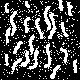
\includegraphics[width=2.0cm]{images/worms80.png}};
            \node[visible on=<2->] (er) at (3.5,1.2) {
\includegraphics[width=2.0cm]{images/worms80_erode.png}};
            \node[visible on=<4->] (di) at (3.5,-1.2) {
\includegraphics[width=2.0cm]{images/worms80_dilate.png}};
            \node[visible on=<3->] (op) at (7,1.2) {
\includegraphics[width=2.0cm]{images/worms80_open.png}};
            \node[visible on=<4->] (cl) at (7,-1.2) {
\includegraphics[width=2.0cm]{images/worms80_close.png}};
            \node[visible on=<1->] at (or.west)[xshift=-0.3cm] {$u = $};
            \node[visible on=<3->] at (op.east)[xshift=0.7cm] {$= u \open \Bn$};
            \node[visible on=<4->] at (cl.east)[xshift=0.7cm] {$= u \close \Bn$};
            \draw[|->,visible on=<2->] (or) to node[above,yshift=0.5ex] {$\erode \B$} (er);
            \draw[|->,visible on=<4->] (or) to node[below,yshift=-0.5ex] {$\dilate \B$} (di);
            \draw[|->,visible on=<3->] (er) to node[above] {$\dilate \Bm$} (op);
            \draw[|->,visible on=<4->] (di) to node[below] {$\erode \Bm$} (cl);
        \end{tikzpicture}
    \end{center}
\end{frame}

\subsection{Top-hat Filter}

\begin{frame}
    \frametitle{Definition der Top-hat Filter}
    \pause
    \begin{definition}
        Definiere den \emph{White-top-hat Operator}
        \begin{math}
            u \wtophat B := u - u \open B
        \end{math}
        und den \emph{Black-top-hat Operator}
        \begin{math}
            u \btophat B := u \close B - u.
        \end{math}
    \end{definition}
    \pause
    \begin{itemize}
        \item
            „$u \wtophat B$ extrahiert helle Strukturen kleiner als $B$“
        \item
            „$u \btophat B$ extrahiert dunkle Strukturen kleiner als $B$“
    \end{itemize}
\end{frame}

\begin{frame}
    \frametitle{Eigenschaften der Top-hat Filter}
    \begin{definition}
        White-top-hat und Black-top-hat besitzen die Eigenschaften
        \begin{itemize}
            \item
                \emph{Komplementarität}: $u \wbtophat B = \complement u \bwtophat B$,
            \item
                \emph{Translationsinvarianz}: $u^p \wbtophat B = (u \wbtophat B)^p$,
            \item
                \emph{Translationsinvarianz bezüglich des Strukturelements}: $u \wbtophat B = u \wbtophat (B + p)$,
        \end{itemize}
        Falls $|B|$ endlich ist, gilt für den White-top-hat Operator
        \begin{itemize}
            \item
                \emph{Idempotenz}: $(u \wtophat B) \wtophat B = u \wtophat B$.
        \end{itemize}
    \end{definition}
\end{frame}

\begin{frame}
    \frametitle{Anwendung: Begleichen von Beleuchtungsunterschieden}
    \DeclareDocumentCommand{\B}{}{
        \,
        \begin{tikzpicture}[scale=0.05,centerbase,-=]
            \draw[fill=black!30] (0,0) rectangle (10,10);
            \draw (0,0) grid (10,10);
            %\fill (0.5,1.5) circle[radius=0.1];
        \end{tikzpicture}
    }
    \usetikzlibrary{decorations.pathmorphing}
    \begin{center}
        \begin{tikzpicture}[scale=0.8]
            \node (or) at (0,1.5) {
\includegraphics[width=2.2cm]{images/leopard250.png}};
            \node at (or.west)[xshift=-1.2cm] {$B = \B, \; u = $};
            \node[visible on=<2->] (ort) at (5,1.5) {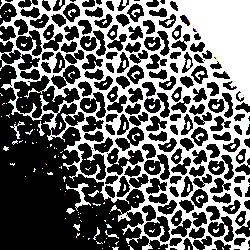
\includegraphics[width=2.2cm]{images/leopard250_thres.png}};
            \node[visible on=<3-5>] (cl) at (-3,-1.5) {
\includegraphics[width=2.2cm]{images/leopard250_close.png}};
            \node[visible on=<3-5>] at (cl.south)[yshift=-0.2cm] {$u \close B$};
            \node[visible on=<4-5>] (bt) at (0,-1.5) {
\includegraphics[width=2.2cm]{images/leopard250_btophat.png}};
            \node[visible on=<4-5>] at (bt.south)[yshift=-0.2cm] {$u \btophat B$};
            \node[visible on=<5>] (btt) at (5,-1.5) {
\includegraphics[width=2.2cm]{images/leopard250_btophat_thres.png}};
            \node[visible on=<7->] (op) at (-3,-1.5) {
\includegraphics[width=2.2cm]{images/leopard250_open.png}};
            \node[visible on=<7->] at (op.south)[yshift=-0.2cm] {$u \open B$};
            \node[visible on=<8->] (wt) at (0,-1.5) {
\includegraphics[width=2.2cm]{images/leopard250_wtophat.png}};
            \node[visible on=<8->] at (wt.south)[yshift=-0.2cm] {$u \wtophat B$};
            \node[visible on=<9->] (wtt) at (5,-1.5) {
\includegraphics[width=2.2cm]{images/leopard250_wtophat_thres.png}};
            \draw[->,visible on=<2->] (or) to (ort);
            \draw[->,visible on=<5>] (bt) to (btt);
            \draw[->,visible on=<9>] (wt) to (wtt);
        \end{tikzpicture}
    \end{center}
\end{frame}

\subsection{Hit-or-Miss Operator}

\begin{frame}
    \frametitle{Definition des Hit-or-Miss Filters}
    \pause
    \begin{definition}
        Für ein Bild $u$ und zwei Strukturelemente $B, C \subset \Omega$ definiere den \emph{Hit-or-Miss Filter}
        \begin{math}
            u \hitormiss (B,C) := (u \erode B) \wedge (\complement u \erode C).
        \end{math}
    \end{definition}
\end{frame}

\begin{frame}
    \frametitle{Beispiel: Erkennen von Ecken}
    \DeclareDocumentCommand{\B}{}{
        %\,
        \begin{tikzpicture}[scale=0.20,centerbase,-=]
            \draw[gray,ultra thin] (0,0) grid (3,3);
            \draw[fill=black!30] (1,0) rectangle (2,1);
            \draw[fill=black!30] (1,1) rectangle (2,2);
            \draw[fill=black!30] (2,1) rectangle (3,2);
            \fill (1.5,1.5) circle[radius=0.1];
        \end{tikzpicture}
    }
    \DeclareDocumentCommand{\C}{}{
        %\,
        \begin{tikzpicture}[scale=0.20,centerbase,-=]
            \draw[gray,ultra thin] (0,0) grid (3,3);
            \draw[fill=black!30] (0,0) rectangle (1,1);
            \draw[fill=black!30] (0,1) rectangle (1,2);
            \draw[fill=black!30] (1,2) rectangle (2,3);
            \draw[fill=black!30] (2,2) rectangle (3,3);
            \fill (1.5,1.5) circle[radius=0.1];
        \end{tikzpicture}
    }
    \begin{center}
        \begin{tikzpicture}
            \node (or) at (0,0) {
\includegraphics[width=3.0cm]{images/rects.png}};
            \node[visible on=<2->] at (or.east)[xshift=1.44cm] {$ \hitormiss \; \Big(\B, \C\Big) = $};
            \node[visible on=<3->] (hm) at (6.2,0) {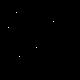
\includegraphics[width=3.0cm]{images/rects_hitmiss.png}};
        \end{tikzpicture}
    \end{center}
\end{frame}

\subsection{Rangordnungs-Filter}

\begin{frame}
    \frametitle{Definition des Rangordnungs-Filters}
    \pause
    \begin{definition}
        Sei $B$ ein Strukturelement mit $|B| = n \in \N$ Elementen und $\sort(u(x+B)) \in F^n$ für $x \in \Omega$ ein aufsteigend sortierter Vektor der Grauwerte in $u(x+B)$.
        Definiere den \emph{$m$-ten Rangordnungs-Filter}
        \begin{math}
            u \rankorder_m B := \sort(u(x+B))_m.
        \end{math}
    \end{definition}
    \pause
    Es gilt insbesondere $u \rankorder_1 B = u \erode B$ und $u \rankorder_n B = u \dilate B$.
\end{frame}

\begin{frame}
    \frametitle{Definition des Median-Filters}
    \begin{definition}
        Definiere den \emph{Medianfilter}
        \begin{math}
            \med_B(u) := u \rankorder_{\floor{\!\frac{n+1}{2}\!}} B.
        \end{math}
    \end{definition}
\end{frame}

\begin{frame}
    \frametitle{Anwendung: Entfernen von Rauschen}
    \begin{center}
        \begin{tikzpicture}
            \node (or) at (0,0) {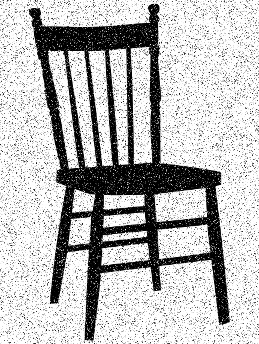
\includegraphics[width=2.2cm,clip,trim=3 3 3 3]{images/chair.png}};
            \node (mm) at (3,0) {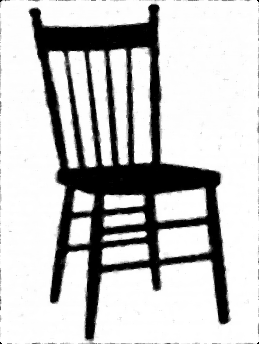
\includegraphics[width=2.2cm,clip,trim=3 3 3 3]{images/chair_morphmedian.png}};
            \node (lm) at (-3,0) {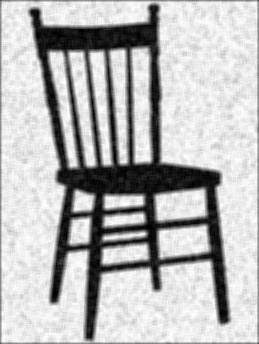
\includegraphics[width=2.2cm,clip,trim=3 3 3 3]{images/chair_linmedian.png}};
            \node[yshift=-0.4em] at (or.south) {$u$};
            \node[align=center,yshift=-1em] at (lm.south) {$u \boxast \tilde B$ \\ (linearer Filter)};
            \node[yshift=-0.4em] at (mm.south) {$\med_B(u)$};
        \end{tikzpicture}
        \begin{math}
            \tilde B &= \frac{1}{25}\Matrix{
                1 & 1 & 1 & 1 & 1 \\
                1 & 1 & 1 & 1 & 1 \\
                1 & 1 & 1 & 1 & 1 \\
                1 & 1 & 1 & 1 & 1 \\
                1 & 1 & 1 & 1 & 1
            },&
            B &= \begin{tikzpicture}[scale=0.23,centerbase,-=]
                \draw[fill=black!30] (0,0) rectangle (5,5);
                \draw (0,0) grid (5,5);
                \fill (2.5,2.5) circle[radius=0.1];
            \end{tikzpicture}
        \end{math}
    \end{center}
\end{frame}

\section{Schlussworte}

\subsection{Einsatzmöglichkeiten}

\begin{frame}
    \frametitle{Denkbare Einsatzmöglichkeiten}
    \pause
    \begin{itemize}
        \item \pause
            Aufarbeitung von Bildern (Scans, Tomographien),
        \item \pause
            Muster-Erkennung/-Suche,
        \item \pause
            Granulometrie,
        \item \pause
            Conway's Game of Life,
        \item
            und weitere \dots
    \end{itemize}
\end{frame}

\subsection{Referenzen}

\begin{frame}
    \frametitle{Referenzen}
    \begin{thebibliography}{}
        \bibitem[Bredies, 2011]{Bredies2011}
        K.~Bredies, D.~Lorenz
        \newblock \emph{Mathematische Bildverarbeitung}
        \newblock Springer, 2011
        \bibitem[Soille, 2004]{Soille2004}
        P.~Soille
        \newblock \emph{Morphological Image Analysis}
        \newblock Springer, 2004
    \end{thebibliography}
    \par\vspace{1em}
    \emph{Alle verwendeten Bilder sind selbst erstellt, oder befinden sich in der Public Domain.}
\end{frame}



\end{document}
